\chapter{Applications}

\section{Rayonnement d'une charge accélérée}
\subsection{Présentation générale}

{\txt On considère une charge (ou un ensemble de charges) en mouvement quelconque, et le but est de déterminer le champ électromagnétique créé dans tout l'espace. Le plus simple est de se placer en jauge de Lorenz ($\nab\cdot\vec{A}+\frac{1}{c^2}\partial_t\phi=0$) et de considérer les équations satisfaites par les potentiels :}
$$
	\left\{ \begin{array}{c@{-}c@{\;}l}
		\nab^2\phi&\frac{1}{c^2}\partial_t^2\phi&=-\frac{\rho}{\epsilon_0}\\
		\nab^2\vec{A}&\frac{1}{c^2}\partial_t^2\vec{A}&=-\mu_0\vec{j}
	\end{array} \right.
$$

Que ce soit pour $\phi$ ou pour n'importe quelle composante cartésienne de $\vec{A}$, l'équation est de la forme
$$
	\nab^2\psi-\frac{1}{c^2}\partial_t^2\psi=-f(\vec{r},t)
$$
qui se résout par la technique des fonctions de Green
$$
	\left(\nab^2-\frac{1}{c^2}\partial_t^2\right)G(\vec{r},t,\vec{r}\,',t')=-\delta(\vec{r}-\vec{r}\,')\delta(t-t')
$$

Comme toute équation aux dérivées partielles, il faut spécifier les conditions aux limites. En l'absence de condition aux limites (\emph{i.e.} une solution dans $\mathbb{R}^3\times\mathbb{R}$) on obtient deux fonctions de Green $G^+$ (retardé) et $G^-$ (avancé).
$$
	G^\pm (\vec{r},t,\vec{r}\,',t')=\frac{1}{4\pi\|\vec{r}-\vec{r}\,'\|}\delta\left(t'-\left(t\mp\frac{\|\vec{r}-\vec{r}\,'\|}{c}\right)\right)
$$

La solution générale se construit à l'aide des fonctions de Green et de la solution de l'équation homogène associée. En l'absence de contribution de l'équation homogène et de la fonction de Green avancée (\emph{i.e.} qu'en $t=+\infty$, il ne reste que la contribution de l'équation homogène), on a,
$$
	\begin{array}{r@{\;}l}
		\psi(\vec{r},t)&=\frac{1}{4\pi}\bigintss \dif t'\,\dif^3 \vec{r}\,'\, 
		\frac{\delta\left(t'-\left(t-\frac{\|\vec{r}-\vec{r}\,'\|}{c}\right)\right)}
			{\|\vec{r}-\vec{r}\,'\|}
		f(\vec{r}\,',t')\\
		&=\frac{1}{4\pi}\bigintsss\dif^3\vec{r}\,'\frac{\left[f(\vec{r}\,',t')\right]_{\text{ret}}}{\|\vec{r}-\vec{r}\,'\|}
	\end{array}
$$
où
$$
	\left[\kern 1em\right]_{\text{ret}} \text{ applique la fonction en } t'=t-\frac{\|\vec{r}-\vec{r}\,'\|}{c}
$$

Dans le cas électromagnétique, on a :..


Cas d'une charge ponctuelle au mouvement quelconque :
$$
	\phi(\vec{r},t)=\frac{1}{4\pi\epsilon_0}\bigintss \dif t'\,\dif^3 \vec{r}\,'\, 
		\frac{\delta\left(t'-\left(t-\frac{\|\vec{r}-\vec{r}\,'\|}{c}\right)\right)}
			{\|\vec{r}-\vec{r}\,'\|}\rho(\vec{r}\,',t')
$$
et
$$
	\rho(\vec{r}\,',t')=q\delta(\vec{r}\,'-\vec{r}_q(t'))
$$
$$
	\begin{array}{r@{\;}l}
		\phi(\vec{r},t)&=\frac{q}{4\pi\epsilon_0}\bigintss \dif t'\,\dif^3 \vec{r}\,'\, 
		\frac{\delta\left(t'-\left(t-\frac{\|\vec{r}-\vec{r}\,'\|}{c}\right)\right)}
			{\|\vec{r}-\vec{r}\,'\|}\delta(\vec{r}\,'-\vec{r}_q(t'))\\
		&=\frac{q}{4\pi\epsilon_0}\bigintss \dif t'\, 
		\frac{\delta\left(t'-\left(t-\frac{\|\vec{r}-\vec{r}_q(t')\|}{c}\right)\right)}
			{\|\vec{r}-\vec{r}_q(t')\|}
	\end{array}
$$


On effectue le changement de variable $t'\longrightarrow s=t'+\frac{\|\vec{r}-\vec{r}_q(t')\|}{c}$
$$
	\dif s=\dif t'+\frac{1}{c}\frac{\dif r}{\dif t'}\dif t' \text{ où } r\defeq\|\vec{r}-\vec{r}_q(t')\|
$$
Alors
$$
	\begin{array}{r@{\;}l}
		\phi(\vec{r},t)&=\frac{q}{4\pi\epsilon_0}\bigintss\dif s\,\frac{\delta(s-t)}{\left(1+\frac{1}{c}\frac{\dif r}{\dif t'}\right)r}\\[10pt]
		&=\frac{q}{4\pi\epsilon_0}\left[\frac{1}{\left(1+\frac{1}{c}\frac{\dif r}{\dif t'}\right)}\right]_{s=t}
	\end{array}
$$
$s=t$ correspond à $t'=t-\frac{\|\vec{r}-\vec{r}_q(t')\|}{c}$, soit à l'instant retardé.
$$
	\begin{array}{r@{\;}l}
		\frac{\dif r}{\dif t'}&=\frac{\dif}{\dif t'}\sqrt{(\vec{r}-\vec{r}_q(t'))^2}\\
			&=-\frac{\dif \vec{r}_q}{\dif t'}\cdot\frac{\vec{r}-\vec{r}_q(t')}{\|\vec{r}-\vec{r}_q(t')\|}\\
			&=-\vec{v}(t')\cdot\vec{n}
	\end{array}
$$
où $\vec{n}=\frac{\vec{r}-\vec{r}_q(t')}{\|\vec{r}-\vec{r}_q(t')\|}$.

Finalement, on obtient les expressions de Liénard-Wiechert :
$$
	\left\{\begin{array}{r@{\;}l}
		\phi(\vec{r},t)&=\frac{1}{4\pi\epsilon_0}\left[\frac{1}{(1-\vec{\beta}\cdot\vec{n})r}\right]_{\text{ret}}\\
		\vec{A}(\vec{r},t)&=\frac{\mu_0}{4\pi}\left[\frac{q}{(1-\vec{\beta}\cdot\vec{n})r}\right]_{\text{ret}}\\
	\end{array}\right.
$$

\begin{remark}
Pour une distribution spatiale de charges en mouvement, il faut tenir compte de $t$ dans le calcul de la contribution des charges au potentiel :
	\begin{figure}[H]
	\centering
	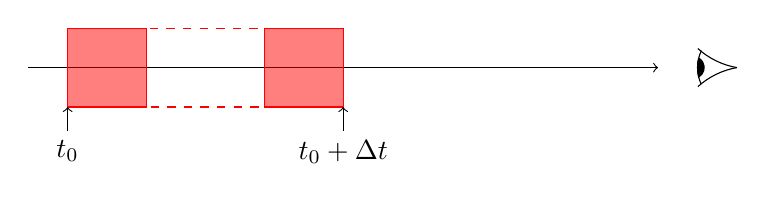
\begin{tikzpicture}
		\draw[->] (0,0) -- (8,0);
		
		\draw[red,fill,fill opacity=0.5] (0.5,-0.5) rectangle (1.5,0.5);
		\draw[red,fill,fill opacity=0.5] (3,-0.5) rectangle (4,0.5);
		\draw[red,dashed] (1.5,0.5) rectangle (3,-0.5);
		
		\draw[<-] (0.5,-0.5) --(0.5,-0.8) node[below] {$t_0$};
		\draw[<-] (4,-0.5) -- (4,-0.8) node[below] {$t_0+\Delta t$};
		
		\begin{scope}[scale=0.5,xshift=18cm]
			\draw (154.5:1) arc (154.5:204.5:1);
			\draw (0,0) arc (260:228:2);
			\draw (0,0) arc (100:132:2);
			\draw[fill=black] (166:1) arc (166:194:1) arc (-60:60:0.28);
		\end{scope}
	\end{tikzpicture}
	\caption*{Charge en déplacement par rapport à un observateur. Sa contribution est délimitée par les pointillés.}
	\end{figure}
Dans la figure précédente, le contribution créée par l'arrière de la charge au moment $t_0$ atteint l'observateur au même moment que la contribution créée par l'avant de la charge au moment $t_0 +\Delta t$.
\end{remark}

On peut écrire les expressions de Liénard-Wiechert sous forme covariante :
$$
	A^\alpha=\frac{\mu_0 c}{4\pi}\left.\frac{qU^\alpha}{U_\beta(x^\beta-x_q^\beta)}\right|_{\tau=\tau_0}
$$
avec 
$$
	U^\alpha=(\gamma c,\gamma\vec{v})
$$
et $\tau_0$ défini par :
$$
	\left(x_\alpha-(x_q)_\alpha(\tau_0)\right)\left(x^\alpha-x_q^\alpha(\tau_0)\right)=0
$$
avec la trajectoire de la particule paramétrée par $\tau$.
$$
	\begin{array}{r@{\;}l}
	\left.U_\beta(r^\beta-r_q^\beta)\right|_{\tau_0}
		&=\gamma c\underbrace{\left(x^0-x_q^0(\tau_0)\right)}_{=\|\vec{r}-\vec{r}_q(\tau_0)\|}
		-\gamma\vec{v}\left(\vec{r}-\vec{r}_q(\tau_0)\right)\\
		&=\gamma c\|\vec{r}-\vec{r}_q(\tau_0)\|\left.(1-\vec{\beta}\cdot\vec{n})\right|_{\tau_0}
	\end{array}
$$
Soit
$$
	\begin{array}{r@{\;}l}
		A^0(r^\lambda)&=\frac{\mu_0 c}{4\pi}\left.\frac{q\gamma c}{\gamma cr(1-\vec{\beta}\cdot\vec{n})}\right|_{\tau_0}\\
			&=\frac{\mu_0 c}{4\pi}\left.\frac{q}{r(1-\vec{\beta}\cdot\vec{n})}\right|_{\tau_0}\\
			&\defeq \frac{\phi}{c}
	\end{array}
$$

On en déduit l'expression des champs :
$$
	\left\{\begin{array}{r@{\;}l}
		\vec{E}(\vec{r},t)&=-\nab\phi-\partial_t\vec{A}=
			\frac{q}{4\pi\epsilon_0}\left(\left[\frac{\vec{n}-\vec{\beta}}{\gamma^2R^2(1-\vec{n}\cdot\vec{\beta})^3}\right]_{\text{ret}}+
			\left[\frac{1}{Rc}\frac{\vec{n}\times((\vec{n}-\vec{\beta})\times\dot{\vec{\beta}}}{(1-\vec{n}\cdot\vec{\beta})}\right]_{\text{ret}}\right)\\
		\vec{B}(\vec{r},t)&=\left[\frac{\vec{n}\times\vec{E}(\vec{r},t)}{c}\right]_{\text{ret}}
	\end{array}\right.
$$
avec
$$
	\begin{array}{l}
		\dot{\vec{\beta}}=\frac{\partial\vec{\beta}}{\partial t'}\\
		R=\|\vec{r}-\vec{r}_q(t')\|\\
		\vec{n}=\frac{\vec{r}-\vec{r}_q}{R}	
	\end{array}
$$

\begin{remarks}\hspace*{1em}
\begin{itemize} \txt
	\item $\vec{n}_{\text{ret}}$, $\vec{E}(\vec{r},t)$ et $\vec{B}(\vec{r},t)$ sont orthogonaux deux à deux.
	 \item On voit apparaître un terme $\dot{\vec{\beta}}$ qui décroit en $\frac{1}{R}$ lorsque $R$ tend vers $+\infty$ (alors que le premier terme décroit en $\frac{1}{R^2}$). C'est le terme dit de rayonnement, associé au caractère accéléré du mouvement, et qui domine le champ à grande distance. C'est ce terme là qui sera l'objet de la suite du cours. On peut en particulier s'intéresser à la puissance totale rayonnée, à sa distribution angulaire, sa distribution spectrale, et aux aspects de polarisation.
	 \item Si $\dot{\vec{\beta}}=\vec{0}$, on retrouve le champ correspondant à une particule en mouvement rectiligne uniforme (\emph{cf.} chapitre 2).
\end{itemize}
\end{remarks}

\subsection{Puissance rayonnée et indicatrice de rayonnement}
\subsubsection{Cas non relativiste}
On considère la limite $\beta\ll 1$. Alors on a :
$$
	\begin{array}{r@{\;}l}
		\vec{E}(\vec{r},t)&=\frac{q}{4\pi\epsilon_0}\left[\frac{1}{Rc}\frac{\vec{n}\times((\vec{n}-\vec{\beta})\times\dot{\vec{\beta}}}{(1-\vec{n}\cdot\vec{\beta})}\right]_{\text{ret}}\\
			&\simeq\frac{q}{4\pi\epsilon_0}\left[\frac{1}{Rc}\frac{\vec{n}\times(\vec{n}\times\dot{\vec{\beta}})}{1}\right]_{\text{ret}}\\
			&=\frac{q}{4\pi\epsilon_0}\left[\frac{(\vec{n}\cdot\dot{\vec{\beta}})\vec{n}-\dot{\vec{\beta}}}{Rc}\right]_{\text{ret}}\\[20pt]
		\vec{B}(\vec{r},t)&=\left[\frac{\vec{n}\times\vec{E}}{c}\right]_{\text{ret}}\\
			&=\frac{q}{4\pi\epsilon_0}\left[\frac{\dot{\vec{\beta}}\times\vec{n}}{Rc^2}\right]_{\text{ret}}\\[20pt]
		\vec{\Pi}(\vec{r},t)&=\frac{\vec{E}\times\vec{B}}{\mu_0}\\
			&=\frac{\vec{E}\times(\vec{n}\times\vec{E})}{\mu_0c}\\
			&=\frac{\|\vec{E}\|^2}{\mu_0c}\vec{n}
	\end{array}
$$

En notant $\mathcal{P}$ la puissance rayonnée, on a :
$$
	\begin{array}{l}
		\dif \mathcal{P}=\vec{\Pi}\cdot\vec{\dif S}\\
		\dif \Omega=\frac{\dif S}{R^2}
	\end{array}
$$
d'où
$$
	\begin{array}{r@{\;}l}
		 \frac{\dif \mathcal{P}}{\dif S}&=\frac{\|\vec{E}\|^2}{\mu_0c}\\
		 	&=\frac{1}{\mu_0c}\frac{q^2}{(4\pi\epsilon_0c)^2}
		 		\left[\frac{(\dot{\vec{\beta}}\cos(\theta)\vec{n}-\dot{\vec{\beta}})^2}{R^2}\right]_{\text{ret}}\\
		 	&=\frac{q^2}{16\pi^2\epsilon_0c}\left[
		 		\frac{\dot{\vec{\beta}}^2\cos^2(\theta)+\dot{\vec{\beta}}^2
		 		-2\dot{\vec{\beta}}\cos(\theta)\cdot\dot{\vec{\beta}}\cos(\theta)}
		 		{R^2}\right]_{\text{ret}}\\
		 	&=\frac{q^2}{16\pi^2\epsilon_0c}\left[
		 		\frac{\dot{\vec{\beta}}^2\sin^2(\theta)}{R^2}\right]_{\text{ret}}\\
		 	&=\frac{q^2}{16\pi^2\epsilon_0c^3}\left[
		 		\frac{\dot{\vec{v}}^2\sin^2(\theta)}{R^2}\right]_{\text{ret}}\\[15pt]
		 	\multicolumn{2}{l}{\boxed{\frac{\dif \mathcal{P}}{\dif \Omega}=\frac{q^2}{16\pi^2\epsilon_0c^3}\left[
		 		\dot{\vec{v}}^2\sin^2(\theta)\right]_{\text{ret}}}}
	\end{array}
$$

On en déduit la puissance totale rayonnée :
$$
	\begin{array}{r@{\;}l}
		\mathcal{P}_\text{tot}&=\bigintsss_0^{2\pi}\!\dif\phi\bigintsss_0^\pi\!\dif\theta\sin(\theta)\frac{\dif\mathcal{P}}{\dif\Omega}\\
			&=2\pi\frac{4}{3}\frac{q^2\dot{\vec{v}}^2}{16\pi^2\epsilon_0c^3}\\[15pt]
			\multicolumn{2}{l}{\boxed{\mathcal{P_\text{tot}}=\frac{q^2\dot{\vec{v}}^2}{6\pi\epsilon_0c^3}}}
	\end{array}
$$
On obtient la formule de Larmor. $\dot{\vec{v}}$ désigne ici $\dot{\vec{v}}_\text{ret}$.

L'indicatrice de rayonnement est la surface correspondant à $\frac{\dif\mathcal{P}}{\dif S}=\text{cte}$, soit une surface satisfaisant $R=\text{cte}\,\sin(\theta)$.

\begin{figure}[H]
\centering
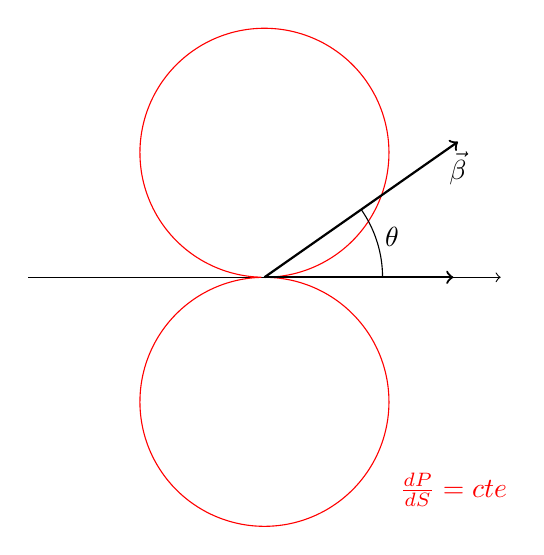
\begin{tikzpicture}[scale=3]
	\draw[->] (-1,0) -- (1,0);
	\draw[color=red,domain=0:360,samples=200,smooth] plot (canvas polar cs:angle=\x,radius={abs(30*sin(\x))});
	\node at (0.8,-0.9) [red]{$\frac{dP}{dS}=cte$};
	\draw [thick,->] (0,0) -- (35:1) node[below]{$\vec{\beta}$};
	\draw [thick,->] (0,0) -- (0.8,0);
	\draw (0:0.5) arc (0:35:0.5);
	\node at (20:0.5)[right]{$\theta$};
\end{tikzpicture}
\caption*{Indicatrice de rayonnement}
\end{figure}

\subsubsection{Cas relativiste}

L'énergie qui est reçue entre les instants $t$ et $t+\dif t$ a été émise entre les instants $t'$ et $t'+\dif t'$, avec $t=t'+\frac{R(t')}{c}$
$$
	\begin{array}{r@{\;}l}
		t+\dif t&=t'+\dif t'+\frac{R(t'+\dif t')}{c}\\
			&=t'+\dif t'\left(1+\frac{1}{c}\frac{\dif R(t')}{\dif t'}\right)+\frac{R(t')}{c}
	\end{array}
$$
avec
$$
	\frac{\dif R}{\dif t'}=\frac{\dif}{\dif t'}\|\vec{r}-\vec{r}_q(t')\|=-\vec{v}_q(t)\cdot\vec{n}
$$
et
$$
	\vec{n}=\frac{\vec{r}-\vec{r}_q}{\|\vec{r}-\vec{r}_q\|}
$$
soit 
$$
	\dif t = \dif t'\left.(1-\vec{\beta}\cdot\vec{n})\right|_\text{ret}
$$

On s'intéresse à la puissance émise, et on a donc :
$$
	\frac{\dif \mathcal{P}}{\dif S}=\frac{q^2}{16\pi^2\epsilon_0c}\frac{\|\vec{n}\times((\vec{n}-\vec{\beta})\times\dot{\vec{\beta}})\|}{R^2(1-\vec{n}\cdot\vec{\beta})^5}
$$
Soit $\theta=(\dot{\vec{v}},\vec{n})$ et $\psi=(\dot{\vec{\beta}},\vec{\beta})$
$$
	\frac{\dif \mathcal{P}}{\dif S}=...
$$
et
$$
	\mathcal{P}_\text{tot}=\bigintsss_0^{2\pi}\!\dif\phi\bigintsss_0^\pi\!\dif\theta\,\sin(\theta)\frac{\dif\mathcal{P}(t')}{\dif\Omega}
$$

{\txt $\mathcal{P}_\text{tot}$ est un invariant relativiste, et on a donc cherché à donner une formulation covariante de la formule de Larmor en introduisant uniquement $\vec{\beta}$ et $\dot{\vec{\beta}}$}. On s'inspire donc de :
$$
	\text{Larmor : }\mathcal{P_\text{tot}}=\frac{q^2\dot{\vec{v}}^2}{6\pi\epsilon_0c^3}=\frac{q^2}{6\pi\epsilon_0c^3m^2}\dot{\vec{p}}\,^2
$$
car $\vec{p}=m\vec{v}$ en mécanique non relativiste. Considérons l'expression :
$$
	\mathcal{P}_\text{tot}=\frac{q^2}{6\pi\epsilon_0c^3m^2}\frac{\dif p_\mu}{\dif\tau}\frac{\dif p^\mu}{\dif\tau}
$$
avec le quadrivecteur énergie-impulsion
$$
	p^\mu=\left(\frac{E}{c},\vec{p}\right)
$$

$$
	\frac{\dif p^0}{\dif\tau}=\frac{\dif p^0}{\dif t}\frac{\dif t}{\dif \tau}=\gamma\frac{\dif p^0}{\dif t}
$$
avec
$$
	p^0=\frac{E}{c}=\frac{\sqrt{p^2+m^2c^4}}{c}
$$
On a alors :
$$
	\begin{array}{r@{\;}l}
		\frac{\dif E}{\dif t}&=\frac{pc^2}{\sqrt{p^2c^2+m^2c^4}}\frac{\dif p}{\dif t}\\
			&=\beta c\frac{\dif p}{\dif t}
	\end{array}
$$
soit
$$
	\begin{array}{r@{\;}l}
		\mathcal{P}_\text{tot}&=\frac{q^2}{6\pi\epsilon_0m^2c^3}\left(\left(\frac{\dif\vec{p}}{\dif\tau}\right)^{\!\!2}-\beta^2\left(\frac{\dif\vec{p}}{\dif\tau}\right)^{\!\!2}\right)\\
			&\xrightarrow[\beta\longrightarrow 0]{}\frac{q^2}{6\pi\epsilon_0m^2c^3}\left(\frac{\dif\vec{p}}{\dif\tau}\right)^{\!\!2}\\
			&=\frac{q^2}{6\pi\epsilon_0m^2c^3}\left(\frac{\dif\vec{p}}{\dif t}\right)^{\!\!2}
	\end{array}
$$
\vspace{1cm}
$$
	\begin{array}{r@{\;}l}
		\frac{\dif p^0}{\dif\tau}&=\frac{\dif p^0}{\dif t}\frac{\dif t}{\dif\tau}\\
			&=\gamma\frac{\dif p^0}{\dif t}\\
			&=\gamma mc\frac{\dif\gamma}{\dif t}\\
			&=\gamma mc\gamma^3\vec{\beta}\cdot\dot{\vec{\beta}}
	\end{array}
$$
\vspace{1cm}
$$
	\begin{array}{r@{\;}l}
		\frac{\dif\gamma m\vec{v}}{\dif \tau}&=\gamma\frac{\dif\gamma m\vec{v}}{\dif t}\\
			&=\gamma m\vec{v}\frac{\dif\gamma}{\dif t}+\gamma^2m\frac{\dif\vec{v}}{\dif t}\\
			&=\gamma^4m\vec{v}(\vec{\beta}\cdot\dot{\vec{\beta}})+\gamma^2mc\dot{\vec{\beta}}
	\end{array}
$$
d'où
$$
	\begin{array}{r@{\;}l}
		\mathcal{P}_\text{tot}&=-\frac{q^2}{6\pi\epsilon_0m^2c^2}\left(
			\gamma^8m^2c^2(\vec{\beta}\cdot\dot{\vec{\beta}})^2
			-(\gamma^2mc)^2(\gamma^2\vec{\beta}(\vec{\beta}\cdot\dot{\vec{\beta}})+\dot{\vec{\beta}})^2
			\right)\\
		&=\frac{q^2}{6\pi\epsilon_0c}\left(
			\gamma^4\left(\gamma^2\vec{\beta}(\vec{\beta}\cdot\dot{\vec{\beta}})+\dot{\vec{\beta}}\right)^2
			-\gamma^8(\vec{\beta}\cdot\dot{\vec{\beta}})^2\right)\\
		&=\frac{q^2}{6\pi\epsilon_0c}\left(\gamma^6(\vec{\beta}\cdot\dot{\vec{\beta}})^2
			+\gamma^4\dot{\vec{\beta}}^2\right)\\
		&=\frac{q^2}{6\pi\epsilon_0c}\gamma^6\dot{\vec{\beta}}\,^2\left(
			1-\beta^2\sin^2(\psi)\right)\\
		\multicolumn{2}{l}{\boxed{\mathcal{P}_\text{tot}=\gamma^6\left(\dot{\vec{\beta}}\,^2-
			(\vec{\beta}\times\dot{\vec{\beta}})^2\right)}}
	\end{array}
$$
On a donc bien trouvé une expression covariante de $\mathcal{P}_\text{tot}$.

\begin{remark}
En général, on ne contrôle pas (via la force de Lorentz) $\vec{\beta}$ et $\dot{\vec{\beta}}$, mais $\vec{p}$ et $\dot{\vec{p}}$. On réexprime ces formules en faisant apparaître l'impulsion.
\end{remark}